\documentclass[12pt]{report}
\usepackage{graphicx}
\usepackage{listings}

\title{Gain Shell Access to Metasploitable}
\author{Gunnar Holwerda}
\date{February 3, 2015}
\renewcommand*\contentsname{Table of Contents}
\newcommand{\mychapter}[2]{
    \setcounter{chapter}{#1}
    \setcounter{section}{0}
    \chapter*{#2}
    \addcontentsline{toc}{chapter}{#2}
}

\begin{document}
\maketitle

\tableofcontents
\clearpage

\mychapter{1}{Executive Summary}
\section{Executive Summary}
I was tasked with exploiting the Metasploitable virtual machine and finding a way to get shell access.
Tools built into Kali Linux were able to help me achieve this, along with the use of the Nessus software.
I started with a basic network scan of the VM and decided to try to use MySQL to gain shell access to the system.
Through trial and error I was able to gather information about the users on the system through the MySQL console.
Since I was able to log into the root account of MySQL I could have accessed many of the other databases held on the system, 
but I chose to focus on the MySQL database, specifically the User database. Although nothing was there I moved on and just downloaded the ``/etc/password''
file and used it as a userlist to brute force into an ssh account.
\clearpage

\mychapter{2}{Attack Narrative}
\section{Exploration}
I started with an nmap of the ip address:
	\begin{verbatim}
	# nmap 192.168.2.12
	\end{verbatim}
Which gave me a list of available ports:\\
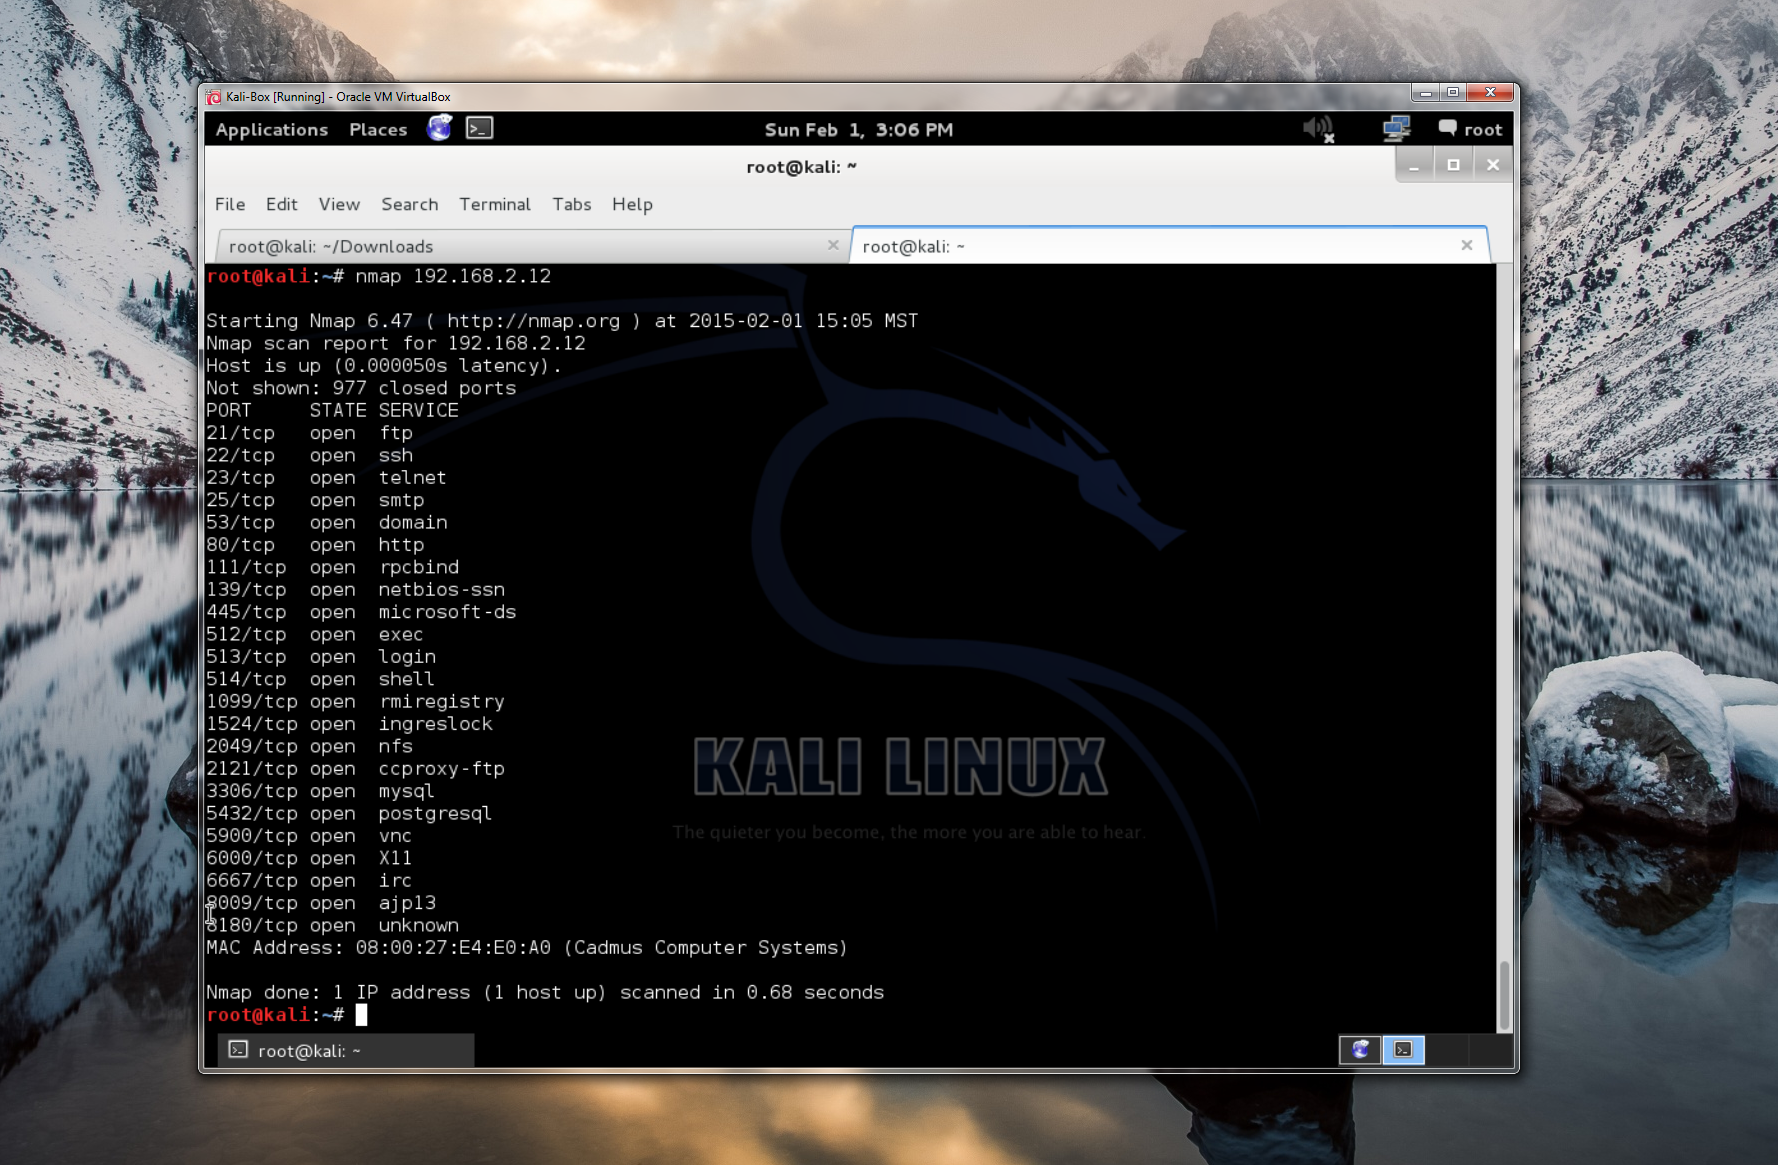
\includegraphics[scale=0.33, width=\linewidth]{list_of_ports.PNG}
\newline
I decided that I would try to investigate the MySQL port and see if that could give me any sort of access to the system. I decided to run an NetCat on the port:
	\begin{verbatim}
	# ncat 192.168.2.12 3306
	\end{verbatim}
This gave me some very weird output that I could not understand. It was at this point I decided to wait until Nessus finished installing. Then I could run a basic network scan of the system and see if there were any MySQL vulnerabilities on the system.\\
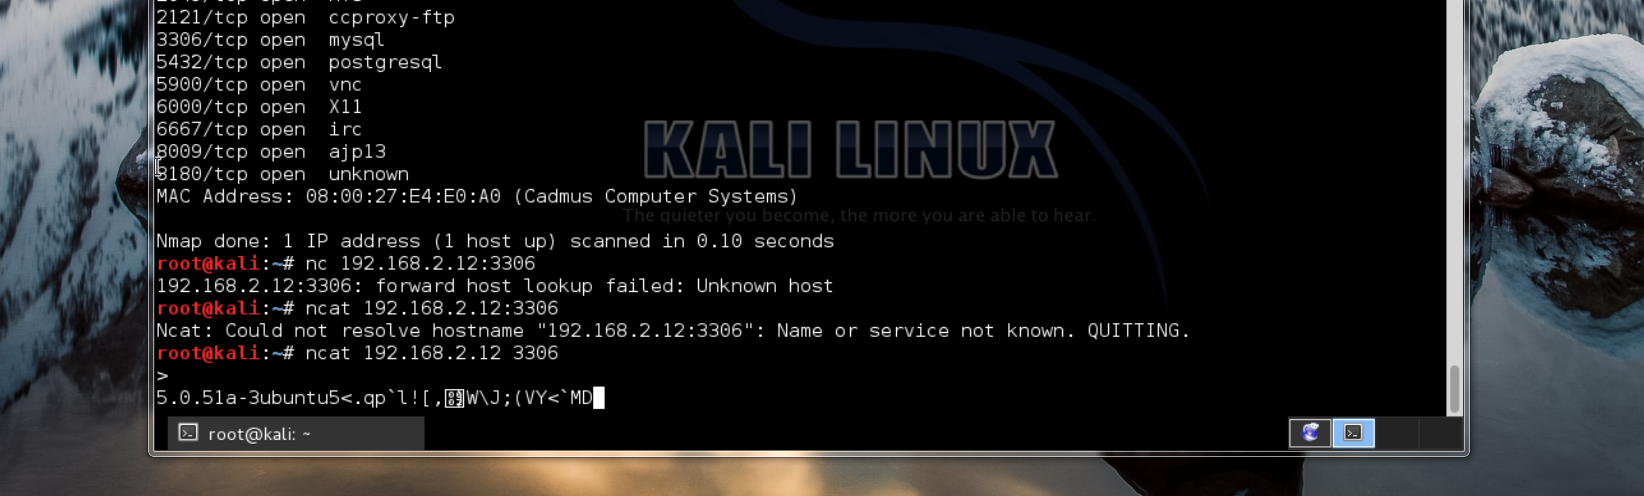
\includegraphics[scale=0.33, width=\linewidth]{ncat_sql_return_info.PNG}
\newline

\section{Nessus Scan}
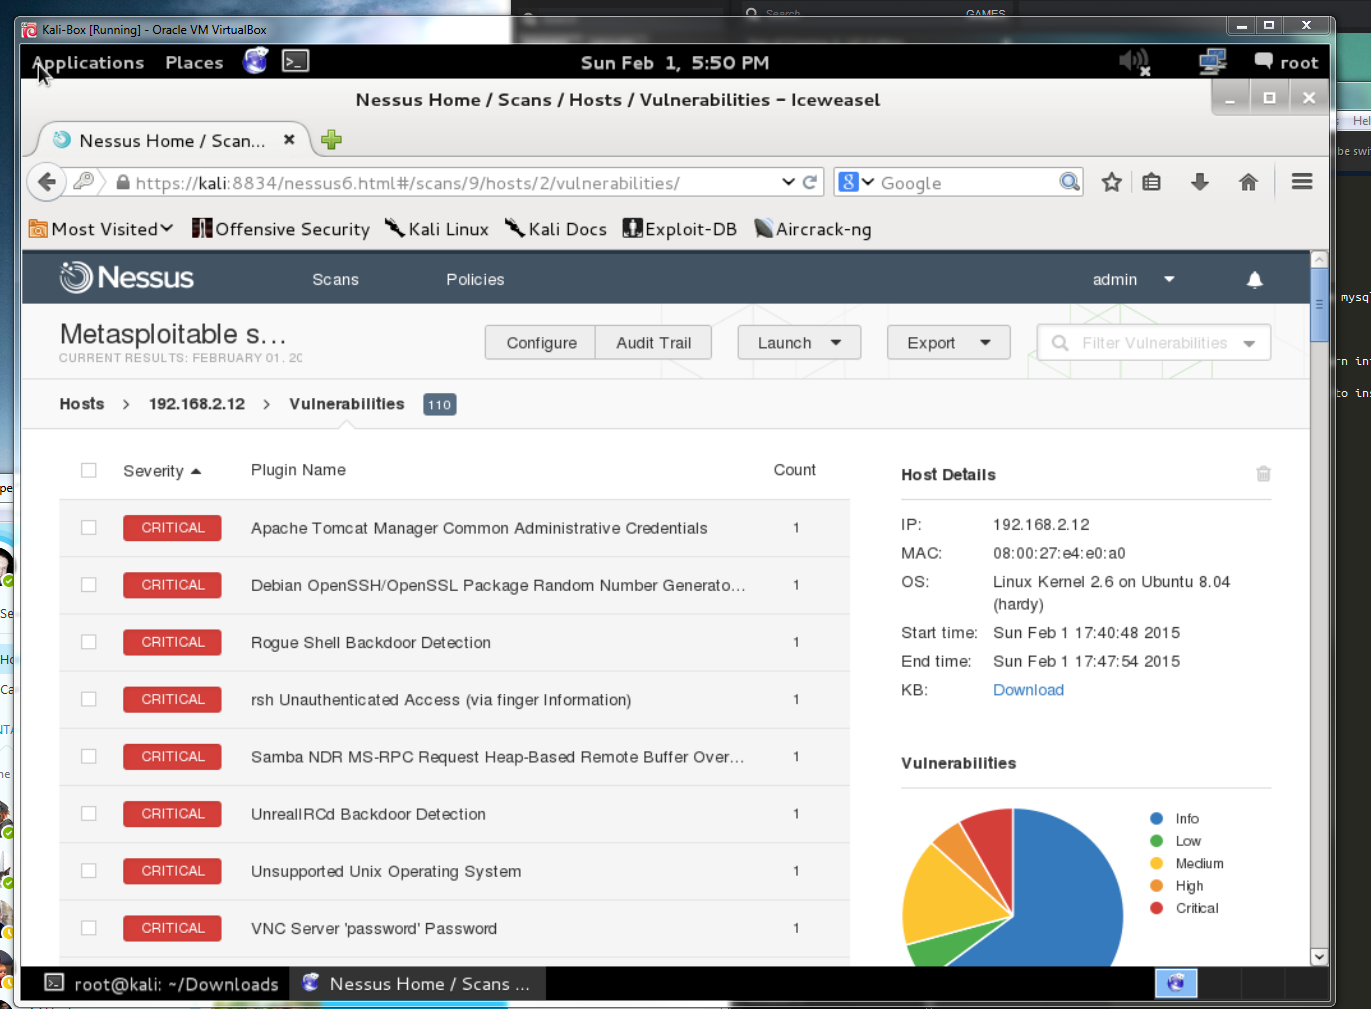
\includegraphics[scale=0.33, width=\linewidth]{nessus_scan.PNG}
The Nessus scan of the virtual machine returned many errors, but since I was interested in attacking the MySQL service I started to check if there were any errors associated with it. I was able to find a vulnerability associated with MySQL of ``MySQL Unpassworded Account Check''.\\
After finding this vulnerability I decided that it was time to load up msfconsole and start to try to exploit it. After searching for MySQL I was able to find a tool called ``mysql\_login''. I decided to try it out as I figured I would try to login to the MySQL service using a blank password like Nessus suggested there was. 
	\begin{verbatim}
	> use auxiliary/scanner/mysql/mysql_login
	> info
	> set RHOSTS 192.168.2.12
	> set BLANK_PASSWORDS true
	> exploit
	\end{verbatim}
After running the tool with the options set as above, I received the output:\
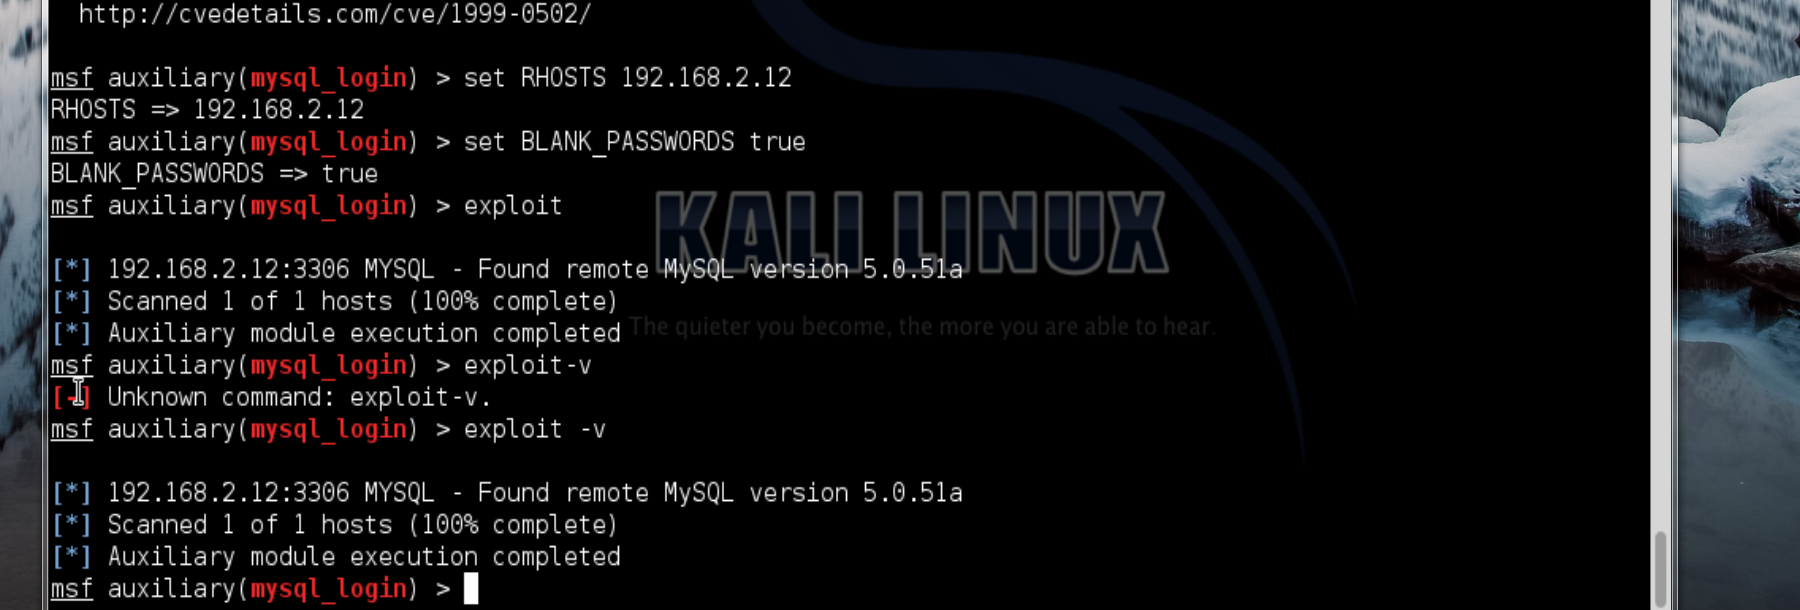
\includegraphics[scale=0.33, width=\linewidth]{blank_password_check_output.PNG}
\newline
I was confused at first as I had thought that Nessus had said the password was blank. Then I remembered that I had forgotten to set a username, so I set the username to root and ran it again:
	\begin{verbatim}
	> set USERNAME root
	> exploit
	\end{verbatim}
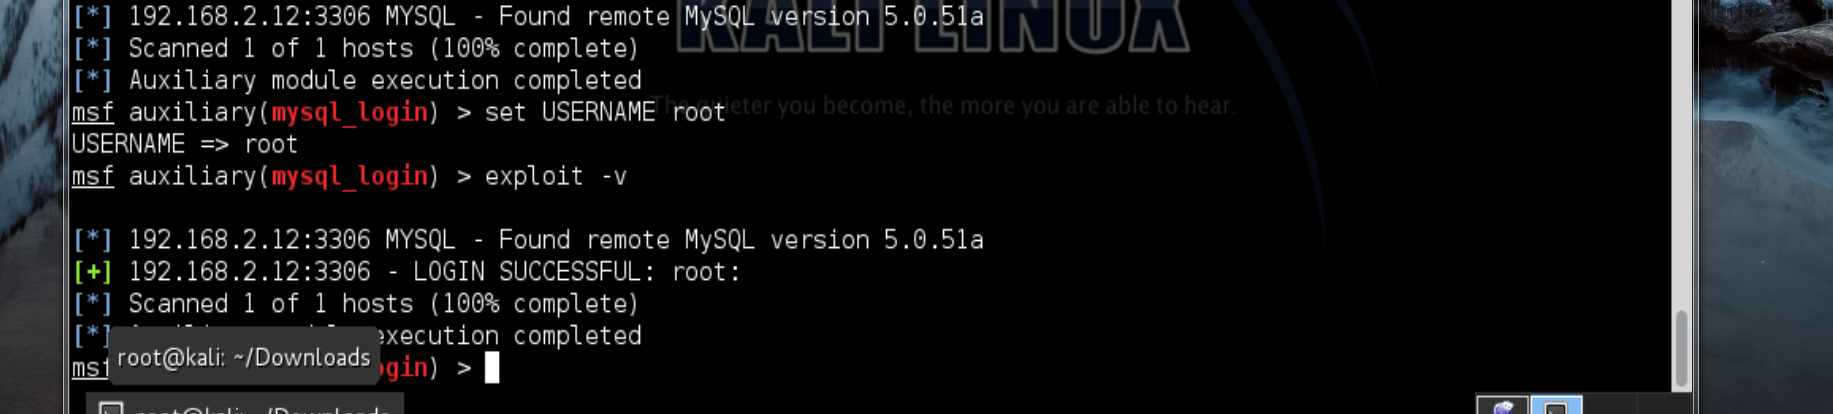
\includegraphics[scale=0.33, width=\linewidth]{success.PNG}
\newline
\section{MySQL}
I now have the username and password to the MySQL service. I decided to attempt to log into the service remotely through my machine to see what I could do from there:
	\begin{verbatim}
	# mysql -h 192.168.2.12 -u root -p
	\end{verbatim}
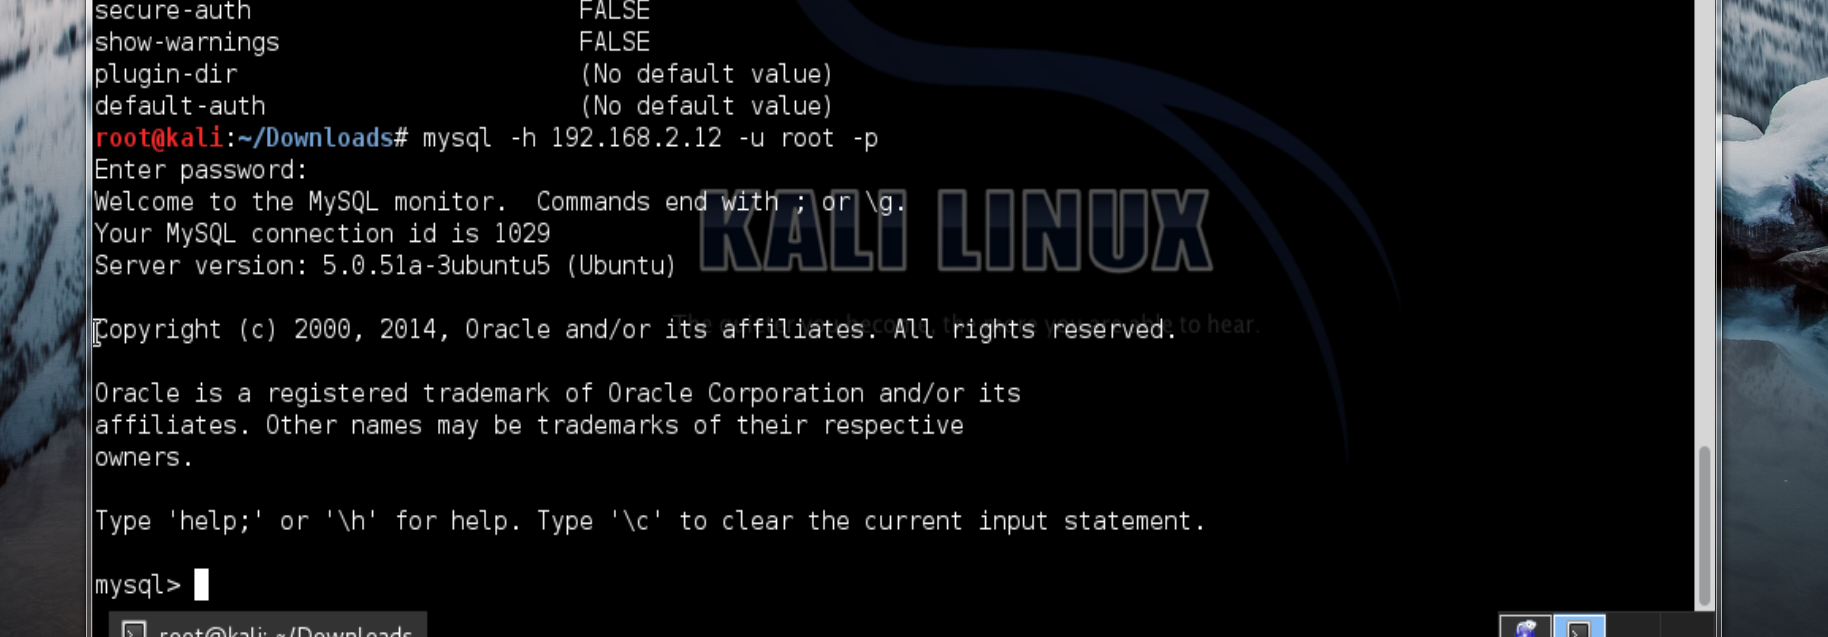
\includegraphics[scale=0.33, width=\linewidth]{successful_sql_login.PNG}
\newline
I ran a ``show grants;'' to find out how much power the user I now controlled has. Turns out I had access to everything in MySQL! What if I tried to open the ``/etc/passwd'' file?\\
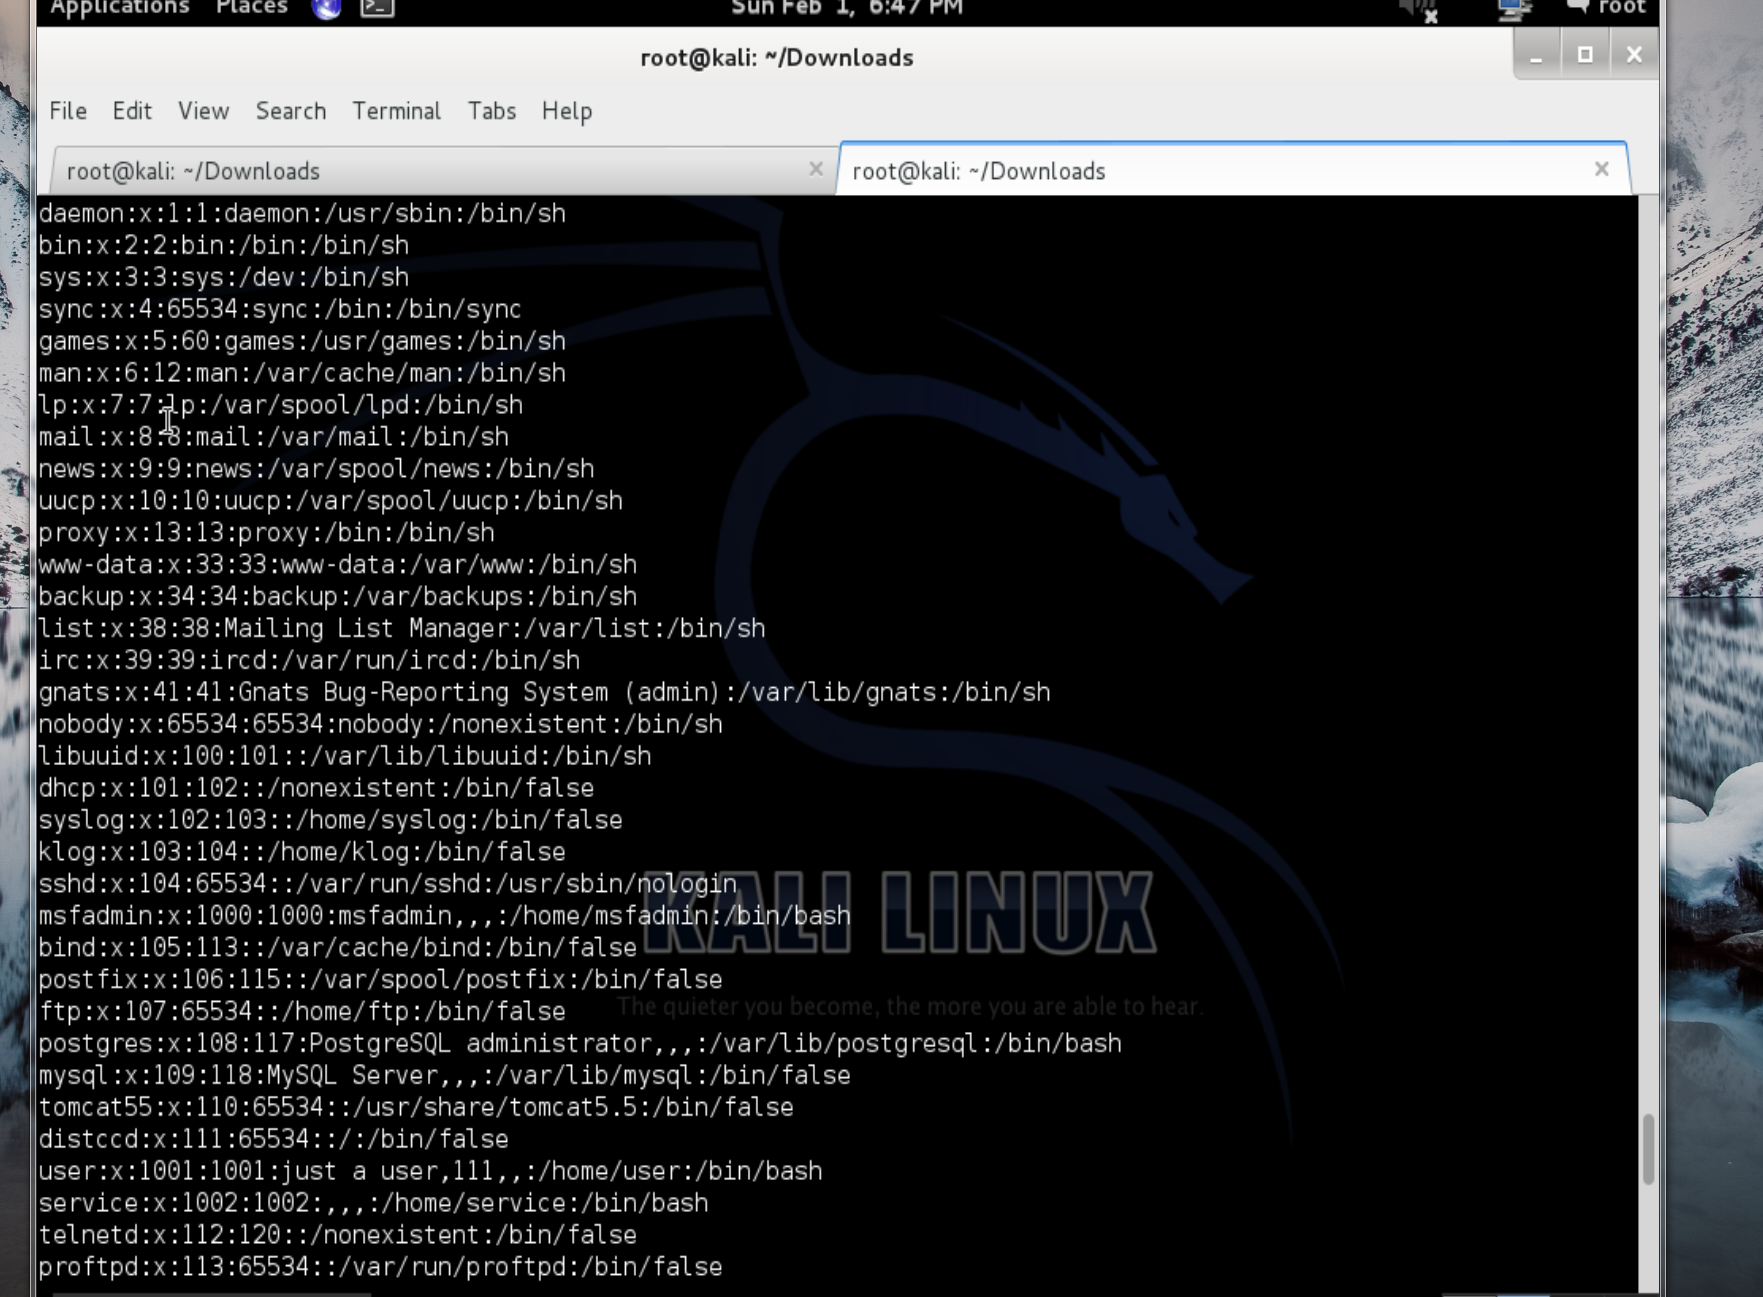
\includegraphics[scale=0.33, width=\linewidth]{_etc_password.PNG}
\newline
I was able to get the file, so now I have a list of users and what group they belong to on the system. I attempted to get the ``/etc/shadow'' file, but was rejected. So this still leaves me with no ability to get into a shell. Now I decided that I would try to investigate the datbases contained within the system to see if there was any information contained within in them that could help me out.
	\begin{verbatim}
	> show databases;
	> use mysql; 
	> Select *;
	> show tables;
	> select * from user;
	> select User from user;
	> select User, Password from user;
	\end{verbatim}
When I selected everything from the user table, I got a very messy printout of the table (see screenshot below). I was able to determine that the table contained a username and password, so I selected both of those from the table. Unfortunately the passwords were not in the table.\\
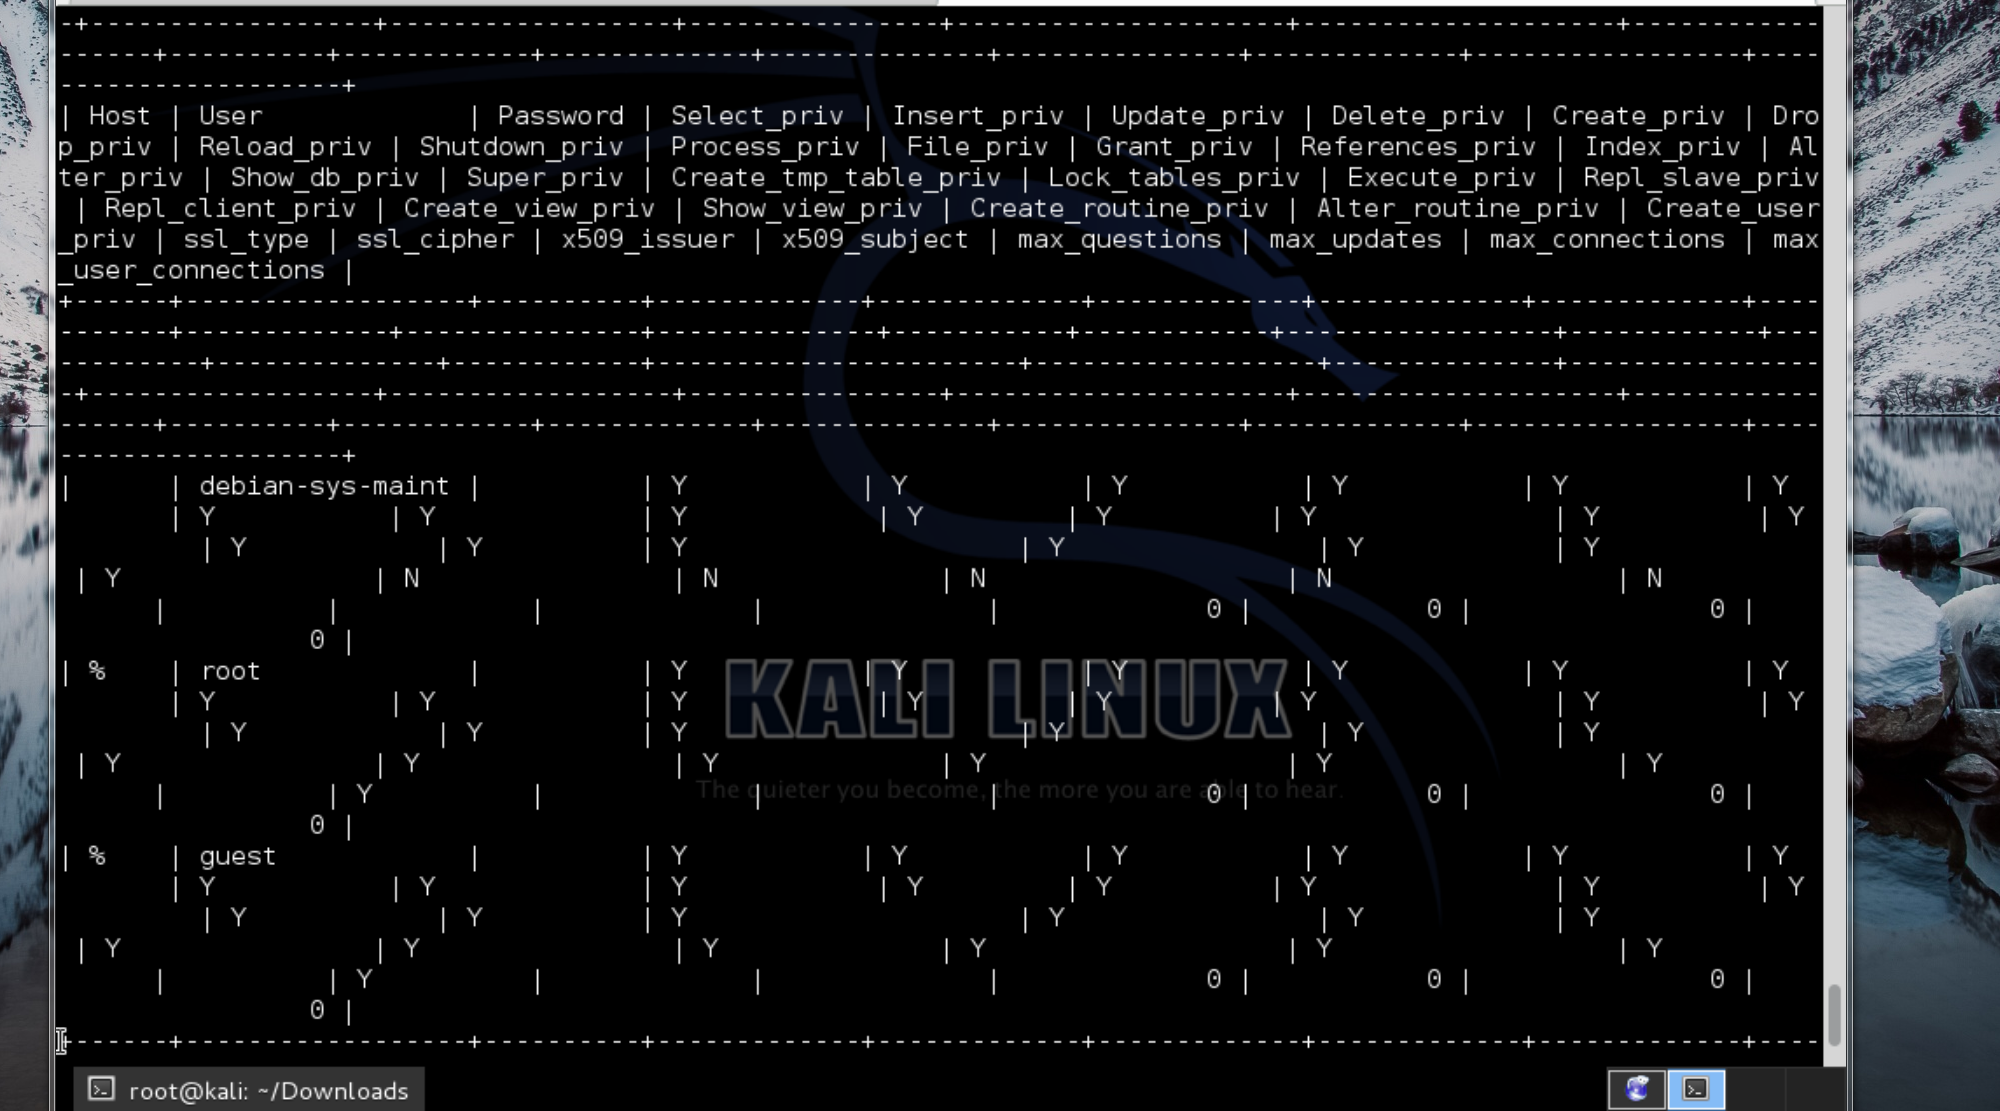
\includegraphics[scale=0.33, width=\linewidth]{weird_output.PNG}
\newline
I then attempted to try to use the mysql\_hashdump tool from msfconsole, unfortunately it was unable to provide me with anything. Next I decided to see if there were any known exploits for the current MySQL version that was running on the system. That search turned up nothing as well. I went into MySQL again and grabbed the print out of the ``/etc/passwd'' file from before to use it as a user list to try to brute force an SSH account.
\newline
\section{SSH}
I determined that I was going to try to brute force an SSH account using the users from the ``/etc/passwd'' file I was able to print out from MySQL. AFter waiting for a long time as Hydra attempted to test multiple passwords for the large user list, I decided to just focus on one user. I picked the user ``user'' and decided to try to brute force it using the namelist.txt wordlist from ``/usr/share/wordlists/metasploit/'' built into Kali. 
	\begin{verbatim}
	# hydra ssh://192.168.2.12 -l user -P /usr/share/wordlists/metasploit/namelist.txt -v -t 8
	\end{verbatim}
\includegraphics[scale=0.33, width=\linewidth]{find_the_login.PNG}
\newline
I was able to successfully find the password for ``user'' and thus login to an SSH account with shell access.
\clearpage

\mychapter{3}{Conclusion}
\section{Conclustion}
In the end I was able to obtain shell access remotely through using msfconsole and Nessus. There are obviously much easier routes to getting a remote shell from the metasploitable VM, but I wanted a challenge so I chose to try to use MySQL as my gateway to gaining access. I had hoped there was a clever way to slide through MySQL into a shell, but I was unable to find a way to do so. I ended up gathering a userlist from my access to MySQL and then brute forced my way into a shell. The MySQL password needs to be secured, it is not safe to use a blank password.

\end{document}